%%%%%%%%%%%%%%%%%%%%%%%%%%%%%%%%%%%%%%%%%%%%%%%%%%%%%%%%%%%%%%%%%%%%%%%%%%%%%%%%


%\documentclass[letterpaper, 10pt, conference]{IEEEtran}
\documentclass{beamer}
\usepackage{tikz}
\usetikzlibrary{calc,decorations.markings,arrows, fadings}
\usepackage{tikz-timing}
\usepackage{amsmath}
\usepackage{xifthen}
\usepackage{amsfonts}
\usepackage{tabu}
\usepackage{graphicx,dblfloatfix}
\usepackage[font=small]{caption}
%\usepackage{subcaption}
\usepackage{cite}
\usepackage{placeins}
\usepackage{xspace}
\usepackage{subfiles}
\usepackage{url}
\usepackage[outline]{contour}

\contourlength{0.18em}

\usetheme{Copenhagen}
\usecolortheme{beetle} 
%\setbeamertemplate{navigation symbols}{}
\beamertemplatenavigationsymbolsempty
\setbeamerfont{footline}{series=\scriptsize}
\usefonttheme{structurebold}

\definecolor{beetle@other}{RGB}{207,184,124} %cu gold
%
%Once I break this in to multiple sections, each section will be added with:
%	\subfile{filename}
%In those other files, I have as preamble:
%	\documentclass[main.tex]{subfiles}
%

\title[\textcolor{black}{Low-Cost Omnidirectional Powertrain}]{A Stick-Slip Omnidirectional Powertrain for Low-Cost Swarm Robotics:\\ Mechanism, Calibration, and Control}
\author[{\tt john.klingner@colorado.edu}]{John Klingner, Anshul Kanakia, Nicholas Farrow, Dustin Reishus and Nikolaus Correll}
\institute[]{Department of Computer Science\\University of Colorado Boulder}
\date{}

\newcommand{\Tau}{\boldsymbol{\mathrm{T}}}

\begin{document}
\begin{frame}
	\titlepage
\end{frame}
\begin{frame}{Motivation \& Background}
	\begin{columns}[c]
		\column{0.7\textwidth}
		\begin{itemize}
			\item Stick-slip motion.
				\note[item]<1->{
					\begin{itemize}
						\item Primary goal is to effect motion cheaply.
						\item Uses the impulse forces generated by vibration motors (cost: $\frac{\$0.50}{\mathtext{unit}}$) to "scoot" the robot along.
					\end{itemize}
				}
			\item Previous work.
				\note[item]<1->{
					\begin{itemize}
						\item Has demonstrated the efficacy of this approach for skid steering motion driven by two motors. **CITE** This work determined that a three-motor setup with holonomic drive was infeasible in real robots. **CITE**
						\item We extend this owrk to allow for an omnidirectional powertrain using three motors.
					\end{itemize}
				}
		\end{itemize}
		\column{0.3\textwidth}
		\begin{figure}
			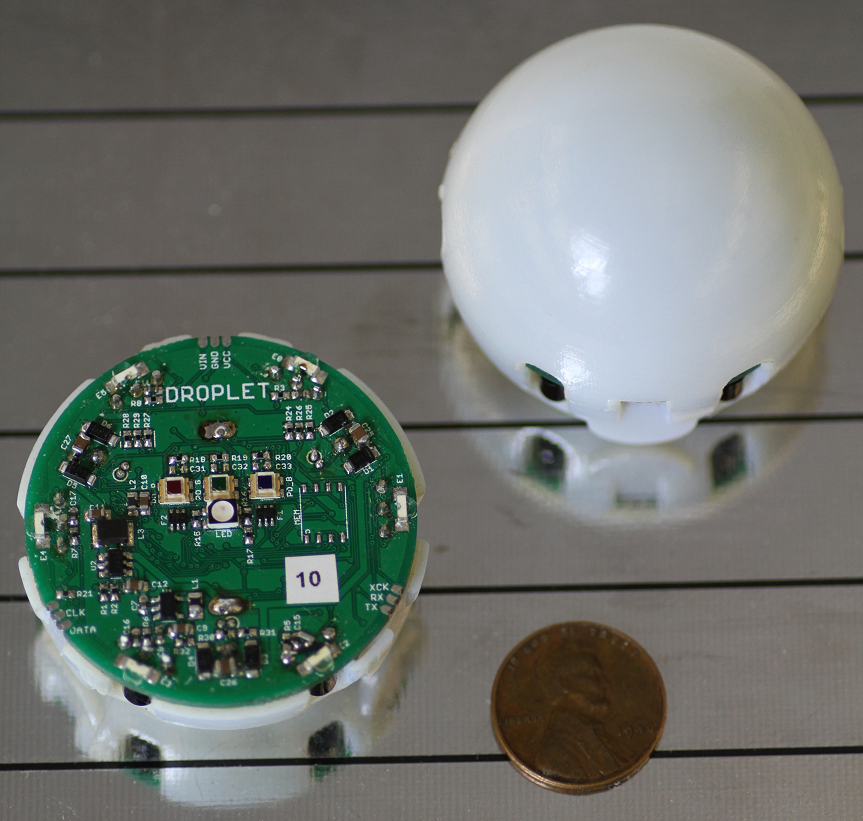
\includegraphics[\linewidth]{Images/droplets.png}
		\end{figure}
		\begin{figure}
			%\subfile{dropletDiagramPresentation}
		\end{figure}
	\end{columns}
\end{frame}
\begin{frame}
	\frametitle{The Method}
	\begin{itemize}
		\item Previous work mounts motors near the legs of the robot. Our method requires that the motors be mounted opposite the legs. **FIGURE** 
		\item The problem observed by previous work was that using three motors at once set up vibrations throughout the robot resulting in instability and uncontrolled motion.	
		\item To avoid this issue, only one motor is ever activated at any given time. **THOUGH I WONDER WHAT HAPPENS IF WE TURN ON TWO AT ONCE?**
		\item One rotation of one motor causes the robot to pivot about the opposite leg, we refer to this as a `step'.
		\item Overall motion is achieved with a sequence of these steps.
	\end{itemize}
\end{frame}
\end{document}